\documentclass[12pt]{article}

% Layout.
\usepackage[top=1.2in, bottom=0.75in, left=1in, right=1in, headheight=1.0in, headsep=0pt]{geometry}

% Fonts.
\usepackage{mathptmx}
\usepackage[scaled=0.86]{helvet}
\renewcommand{\emph}[1]{\textsf{\textbf{#1}}}

% TiKZ.
\usepackage{tikz, pgfplots}
\usetikzlibrary{calc}
\pgfplotsset{my style/.append style={axis x line=middle, axis y line=middle, xlabel={$x$}, ylabel={$y$}}}
\pgfplotsset{compat=1.16}

% Misc packages.
\usepackage{amsmath,amssymb,latexsym,bm,array,multicol,enumitem}
\usepackage{graphicx}
\usepackage{xcolor}

% Commands to set various header/footer components.
\makeatletter
\def\doctitle#1{\gdef\@doctitle{#1}}
\doctitle{Use {\tt\textbackslash doctitle\{MY LABEL\}}.}
\def\docdate#1{\gdef\@docdate{#1}}
\docdate{Use {\tt\textbackslash docdate\{MY DATE\}}.}
\def\doccourse#1{\gdef\@doccourse{#1}}
\let\@doccourse\@empty
\def\docscoring#1{\gdef\@docscoring{#1}}
\let\@docscoring\@empty
\def\docversion#1{\gdef\@docversion{#1}}
\let\@docversion\@empty
\makeatother

% Headers and footers layout.
\makeatletter
\usepackage{fancyhdr}
\pagestyle{fancy}
\fancyhf{} % Clears all headers/footers.
\lhead{\emph{\@doctitle\hfill\@docdate} \medskip
\ifnum \value{page} > 1\relax\else\\
\emph{Name: \rule{3.5in}{1pt}\hfill \@docscoring}
\fi}

\rfoot{\emph{\@docversion}}
\lfoot{\emph{\@doccourse}}
\cfoot{\emph{\thepage}}
\renewcommand{\headrulewidth}{0pt}%
\makeatother

% Paragraph spacing
\parindent 0pt
\parskip 6pt plus 1pt

% A problem is a section-like command. Use \problem{5} for a problem worth 5 points.
\newcounter{probcount}
\newcounter{subprobcount}
\setcounter{probcount}{0}

\newcommand{\problem}[1]{%
\par
\addvspace{4pt}%
\setcounter{subprobcount}{0}%
\stepcounter{probcount}%
\makebox[0pt][r]{\emph{\arabic{probcount}.}\hskip1ex}\emph{[#1 points]}\hskip1ex}

\newcommand{\thesubproblem}{\emph{\alph{subprobcount}.}}

% Subproblems are an enumerate-like environment with a consistent
% numbering scheme.  Use \begin{subproblems}\item...\item...\end{subproblems}
\newenvironment{subproblems}{%
\begin{enumerate}[itemindent=8pt,leftmargin=0pt]%
\setcounter{enumi}{\value{subprobcount}}%
\renewcommand{\labelenumi}{\emph{\textsl{\alph{enumi})}} \,}%
}%
{%
\setcounter{subprobcount}{\value{enumi}}%
\end{enumerate}%
}

% Blanks for answers in normal and math mode.
\newcommand{\blank}[1]{\rule{#1}{0.75pt}}
\newcommand{\mblank}[1]{\underline{\hspace{#1}}}
\def\emptybox(#1,#2){\framebox{\parbox[c][#2]{#1}{\rule{0pt}{0pt}}}}

% Misc.
\renewcommand{\d}{\displaystyle}
\newcommand{\ds}{\displaystyle}
\newcommand{\threeopts}{{\small \hspace{-6mm} $\begin{matrix} \text{\textsc{converges}} \\ \text{\textsc{absolutely}} \end{matrix}$ \qquad\qquad $\begin{matrix} \text{\textsc{converges}} \\ \text{\textsc{conditionally}} \end{matrix}$ \qquad\qquad \textsc{diverges}} \bigskip}


\newcommand{\ba}{\mathbf{a}}
\newcommand{\bb}{\mathbf{b}}
\newcommand{\bc}{\mathbf{c}}
\newcommand{\bi}{\mathbf{i}}
\newcommand{\bj}{\mathbf{j}}
\newcommand{\bk}{\mathbf{k}}
\newcommand{\bu}{\mathbf{u}}
\newcommand{\bv}{\mathbf{v}}
\newcommand{\bw}{\mathbf{w}}

\newcommand{\ip}[2]{\mathrm{\left<#1,#2\right>}}
\newcommand{\vv}[2]{\mathrm{\left<#1,#2\right>}}
\newcommand{\vvv}[3]{\mathrm{\left<#1,#2,#3\right>}}



% Solution boxes.
\usepackage[most]{tcolorbox}
\usepgfplotslibrary{fillbetween}
\definecolor{solbg}{RGB}{225,240,252}
\definecolor{solframe}{RGB}{70,130,180}
\newtcolorbox{solution}[1][]{%
  breakable,
  enhanced,
  colback=solbg,
  colframe=solframe,
  boxrule=0.7pt,
  arc=3pt,
  left=6pt, right=6pt, top=5pt, bottom=5pt,
  before skip=6pt, after skip=6pt,
  fonttitle=\sffamily\bfseries\small,
  coltitle=white,
  title={Solution},
  #1}

\doctitle{Math 252: Quiz 1 --- Solutions}
\docdate{3 September, 2026}
\doccourse{}
\docversion{Solutions}
\docscoring{\fbox{{\LARGE \strut}\hspace{0.8in} / 25}}

\begin{document}
30 minutes maximum.  No aids (book, calculator, etc.) are permitted.
Show all work and use proper notation for full credit.  Answers should
be in reasonably-simplified form.  25 points possible.

\begin{enumerate}
\item Consider the curves $y=x^2$, $y=-x+2$, and $y=0$.
  \begin{enumerate}
  \item (4 points) Sketch the region bounded by these curves. Be sure to clearly
    label the curves and any important points. Show any relevant work.

    \begin{solution}
      First find where the curves meet.

      \emph{Parabola and line:} $x^2 = -x+2 \;\Longrightarrow\; x^2+x-2=0
      \;\Longrightarrow\; (x+2)(x-1)=0$, so $x=-2$ or $x=1$.  Only $x=1$
      borders our region, giving the point $(1,1)$.

      \emph{Parabola and $x$-axis:} $x^2=0$ at the origin, $(0,0)$.

      \emph{Line and $x$-axis:} $-x+2=0$ at $x=2$, giving $(2,0)$.

      \begin{center}
        \vspace{-6pt}
        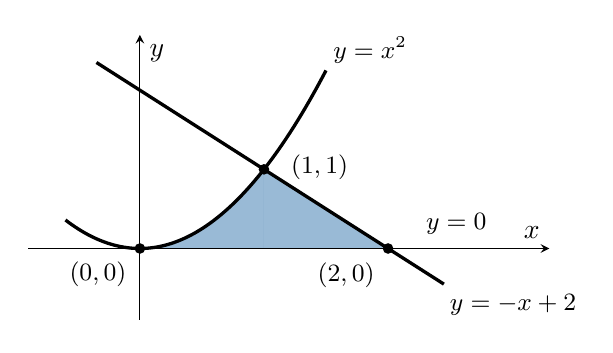
\begin{tikzpicture}
          \begin{axis}[my style, axis on top, width=8.2cm, height=5.2cm,
            xmin=-0.9, xmax=3.3, ymin=-0.9, ymax=2.7,
            xtick=\empty, ytick=\empty, samples=100, clip=false]
            \addplot[draw=none, fill=solframe, fill opacity=0.55, domain=0:1] {x^2} \closedcycle;
            \addplot[draw=none, fill=solframe, fill opacity=0.55, domain=1:2] {2-x} \closedcycle;
            \addplot[very thick, domain=-0.6:1.5] {x^2};
            \addplot[very thick, domain=-0.35:2.45] {2-x};
            \node[anchor=south west, font=\small] at (axis cs:1.48,2.22) {$y=x^2$};
            \node[anchor=north west, font=\small] at (axis cs:2.42,-0.46) {$y=-x+2$};
            \node[anchor=south, font=\small] at (axis cs:2.55,0.05) {$y=0$};
            \addplot[only marks, mark=*, mark size=1.7pt, black] coordinates {(0,0) (1,1) (2,0)};
            \node[anchor=west, font=\small] at (axis cs:1.14,1.03) {$(1,1)$};
            \node[anchor=north east, font=\small] at (axis cs:-0.03,-0.04) {$(0,0)$};
            \node[anchor=north east, font=\small] at (axis cs:1.97,-0.06) {$(2,0)$};
          \end{axis}
        \end{tikzpicture}
      \end{center}
    \end{solution}

  \item (6 points) Find the area of the region bounded by the curves.

    \begin{solution}
      Integrating in $x$, the top curve changes at $x=1$, so the area splits
      into two pieces:
      \[
        A \;=\; \int_0^1 x^2\,dx \;+\; \int_1^2 (-x+2)\,dx .
      \]
      Evaluating each piece,
      \begin{align*}
        \int_0^1 x^2\,dx
          &\;=\; \left[\frac{x^3}{3}\right]_0^1 \;=\; \frac13 ,\\[4pt]
        \int_1^2 (-x+2)\,dx
          &\;=\; \left[-\frac{x^2}{2}+2x\right]_1^2
           \;=\; (-2+4)-\left(-\tfrac12+2\right) \;=\; \frac12 .
      \end{align*}
      Therefore
      \[
        \boxed{\,A \;=\; \frac13+\frac12 \;=\; \frac56\,}.
      \]

      \medskip
      \emph{Alternative (integrating in $y$).}  Here $\sqrt{y}\le x\le 2-y$, so
      \[
        A=\int_0^1\Big[(2-y)-\sqrt{y}\,\Big]dy
        =\left[2y-\frac{y^2}{2}-\frac23 y^{3/2}\right]_0^1
        =2-\frac12-\frac23=\frac56 . \quad\checkmark
      \]
    \end{solution}
  \end{enumerate}

  \newpage

\item Consider the region bounded by the curves $y=x^3$, $y=8$, and
  $x=0$.
  \begin{enumerate}
  \item (4 points) Sketch the region. Be sure to clearly label the curves and any important points. Show any relevant work.

    \begin{solution}
      The curves $y=x^3$ and $y=8$ meet where $x^3=8$, i.e. $x=2$, at the point
      $(2,8)$.  The line $x=0$ meets $y=x^3$ at $(0,0)$ and meets $y=8$ at
      $(0,8)$.

      \begin{center}
        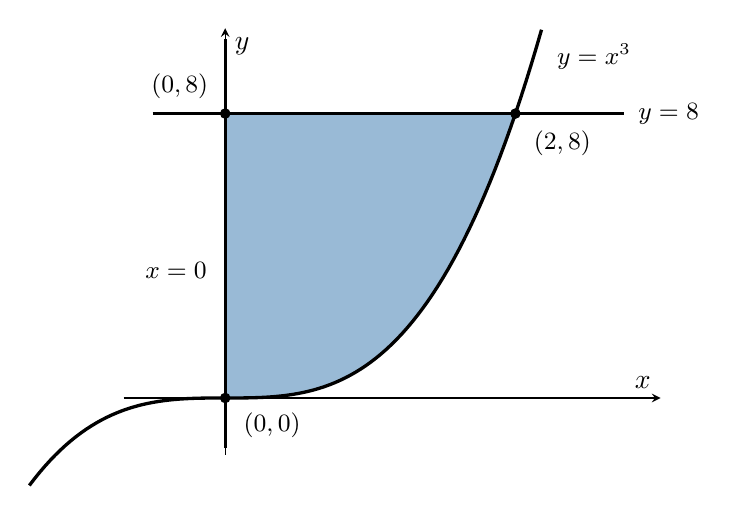
\begin{tikzpicture}
          \begin{axis}[my style, axis on top, width=8.4cm, height=7cm,
            xmin=-0.7, xmax=3.0, ymin=-1.6, ymax=10.4,
            xtick=\empty, ytick=\empty, samples=100, clip=false]
            \addplot[draw=none, name path=curveA, domain=0:2] {x^3};
            \addplot[draw=none, name path=topA, domain=0:2] {8};
            \addplot[draw=none, fill=solframe, fill opacity=0.55]
              fill between[of=curveA and topA];
            \addplot[very thick, domain=-1.35:2.18] {x^3};
            \addplot[very thick, domain=-0.5:2.75] {8};
            \addplot[very thick] coordinates {(0,-1.4) (0,10.1)};
            \node[anchor=west, font=\small] at (axis cs:2.22,9.6) {$y=x^3$};
            \node[anchor=west, font=\small] at (axis cs:2.78,8) {$y=8$};
            \node[anchor=east, font=\small] at (axis cs:-0.06,3.6) {$x=0$};
            \addplot[only marks, mark=*, mark size=1.7pt, black] coordinates {(0,0) (0,8) (2,8)};
            \node[anchor=north west, font=\small] at (axis cs:0.06,-0.15) {$(0,0)$};
            \node[anchor=south east, font=\small] at (axis cs:-0.05,8.15) {$(0,8)$};
            \node[anchor=north west, font=\small] at (axis cs:2.06,7.8) {$(2,8)$};
          \end{axis}
        \end{tikzpicture}
      \end{center}
    \end{solution}

  \item (6 points) Find the volume when the region is rotated around the
    $y$-axis.

    \begin{solution}
      Rotating about the $y$-axis, horizontal slices are perpendicular to the
      axis, so use \emph{disks} in $y$.  At height $y$ the slice runs from
      $x=0$ out to the cubic, $x=y^{1/3}$, so the radius is $R(y)=y^{1/3}$ and
      $y$ runs from $0$ to $8$:
      \begin{align*}
        V &\;=\; \int_0^8 \pi\big(y^{1/3}\big)^2\,dy
             \;=\; \pi\int_0^8 y^{2/3}\,dy \\[4pt]
          &\;=\; \pi\left[\frac35\,y^{5/3}\right]_0^8
             \;=\; \frac{3\pi}{5}\big(8^{5/3}\big)
             \;=\; \frac{3\pi}{5}(32),
      \end{align*}
      so
      \[
        \boxed{\,V=\frac{96\pi}{5}\,}.
      \]

    \end{solution}

  \newpage

  \item (5 points) Set up, but {\bf do not evaluate} an integral that computes
    the volume when the region is rotated around the $x$-axis.

    \begin{solution}
      Now the axis is horizontal, so slice vertically and use \emph{washers} in
      $x$.  At a given $x$ in $[0,2]$ the slice of the region stretches from
      $y=x^3$ up to $y=8$; rotating it about the $x$-axis gives an annulus with
      outer radius $R=8$ and inner radius $r=x^3$:
      \[
        \boxed{\;V=\int_0^2 \pi\Big(8^2-\big(x^3\big)^2\Big)dx
              =\pi\int_0^2\big(64-x^6\big)\,dx\;}
      \]
    \end{solution}
  \end{enumerate}

\end{enumerate}


\end{document}

%-------------------------------------------------------------------------------------------------------------------------------------------------------------------------------------------------------------------

%%% Local Variables:
%%% mode: latex
%%% TeX-master: t
%%% End:
